\documentclass{article}
\usepackage[utf8]{inputenc}
\usepackage{fancyhdr}
\usepackage{graphicx}
\usepackage{geometry}
\usepackage{float}

% ---- Commands ------- %
\newcommand{\documentNumber}[1]{
    \LARGE  \textbf{ Kravspecifikation }
    \\
    \medskip
}
\newcommand{\documentVersion}[1]{
    \medskip
}
\newcommand{\documentTitle}[1]{
    \centerline{\rule{13cm}{0.4pt}}
    \bigskip \bigskip
    \LARGE \textbf{Projekt IDA3} \\
    \bigskip
    \LARGE {#1} \\
    \bigskip \bigskip
    \centerline{\rule{13cm}{0.4pt}}
}

\newcommand{\documentDate}[1]{
    \date {#1} 
}


\renewcommand{\arraystretch}{1.7}  % Vertical padding for tables

\renewcommand{\contentsname}{Innehållsförtäckning}

% --- Header & Footer ---- %
\pagestyle{fancy}
\lhead{\leftmark}
\rhead{}
\rfoot{\thepage}
\cfoot{}
\lfoot{}


% ------------------------------------------------ #

% ----- FILL THIS ----- %
\title {
    \documentNumber {01}    

    % Full name - SHORTNAME
    \documentTitle {Helsingborg Event and Convention Bureau}
    
    % Format: YYYY-MM-DD
    \documentDate {2021-12-03}
    \documentVersion Vv 1.0
    
    \author{Anna Bergvall - Oscar Blixt - Pontus Persson - Filip Sjövall - David Vilppu}
}

\begin{document}
\addtocontents{toc}{\protect\setcounter{tocdepth}{2}}
\maketitle

\thispagestyle{empty}



\newpage

\tableofcontents


\newpage

\section{Dokumenthistoria}
\begin{tabular}{ l | l | l }
    Version & Datum & Beskrivning \\
    \hline
    0.1 & 2021-10-06 & Dokumentet skapat. \\
    0.2 & 2021-11-05 & Första utkast\\
    1.0 & 2021-12-03 & Preliminär inlämning\\
    
\end{tabular}

\section{Introduktion}

    Detta dokument innehåller kraven för ett webbaserat rapporteringssystem som hädanefter benämns som "systemet". Systemet är framtaget och utvecklat på beställning av Helsingborg Convention and Event Bureau (HCEB). Det huvudsakliga syftet med systemet är att Helsingborg stad ska bli miljöcertifierat av GDSM (Global Destination Sustainability Movement) genom att inkorporera deras krav för miljöcertifiering i ett frågeformulär som näringslivet får svara på. Huvudfunktionaliteten är att HCEB ska kunna sammanställa den data som tillkommit till följd av svar på formuläret från näringslivet. Systemet ska intrigeras i en server och det är detta som ska levereras till kunden. I systemet ingår frontend/hemsidan(html, css, javascript), api:n samt databasen. 
    \\\\
    Dokumentets struktureras utifrån prioritering och numrering. Numrering sker enligt \textit{R1} vilka är krav som endast kan hittas i detta dokument, krav med numrering enligt \textit{SF} kommer från scrumboarden. Kraven är prioriterade utefter \textit{stabila krav}, \textit{ändringsbenägna krav} och \textit{uteslutna krav}. 
    

\section{Bakgrund och mål}
                                                                                                                
    \subsection{Mål}
      Helsingborg stad önskar bli certifierade av nätverket Global Destination Sustainability Movement (GDSM), vilket kräver att destinationen varje år skickar in information om hållbarhetsarbetet som utförs av aktörer verksamma inom besöksnäringen i regionen. Syftet med det här projektet är att hjälpa Helsingborg stad att samla in hållbarhetsdata genom att utveckla ett webbaserat frågeformulär som går snabbt och är enkelt att svara på. När datan väl samlats in är det vår uppgift att ta fram en sammanställning som matchar GDSM:s målformat. 
        
    \subsection{Viktiga aktörer}
    Systemet kommer ha två typer av användare:
    \begin{itemize}
        \item \textbf{Svarspersoner:} De personer som jobbar på företagen till vilka frågorna riktar sig. Svarspersonerna kommer att logga in med sin mailadress och svara på formuläret.
        \item \textbf{Admin:} HCEB ska tilldelas rollen administratör och således ha tillgång till en administrationssida där de kan sammanställa årets hållbarhetsdata på ett sätt som matchar GDSM:s målformat och även se enskilda aktörers svar.
     \end{itemize}
    
    \section{Terminologi}
    \begin{itemize}
        \item \textbf{Administratör:} Administratören har tillgång till systemets alla funktioner.
        \item \textbf{Bransch:} Resturanger, hotell, anläggningar samt byråer är de branscher som syftas på.
         \item \textbf{Frågeformulär:} Ett webbaserat system som innehåller frågor med flervalsalternativ samt statistikföring över svaren.
        \item \textbf{HCEB:} Förkortning av Helsingborg Convention and Event Bureau, beställare av systemet.
        \item \textbf{Session:} Data som sparas under tiden som slutanvändaren befinner sig på hemsidan.
        \item \textbf{Svarspersoner:}  De personer som svarar på frågeformuläret, vilka främst arbetar inom besöksnäringen i Helsingborgs stad. 
        \item\textbf{Stabila krav:}  Stabila krav är krav som inte är ändringbenägna - de baseras på funktioner som är grundläggande för att systemet ska möta beställarens behov.
         \item \textbf{Uteslutna krav:}  Krav som inte längre är aktuella.
        \item \textbf{Ändringbenägna krav:}  Krav som sannolikt kommer att förändras eller tas bort.
       
    \end{itemize}
    \newpage
    \section{Hemsidans design}
    
    \subsection{Stabila krav}
    
    T-5 (Från Trello).
     
    \subsection{Ändringsbenägna krav}
    
    \large{\textbf{R1.}}
    \normalsize{Frågeformuläret vilket används av slutanvändarna samt ingår i systemet ska ha ett utseende likt figur 1.}
    
    \begin{figure}[h!]
    \caption{Prototyp över frågeformuläret}
    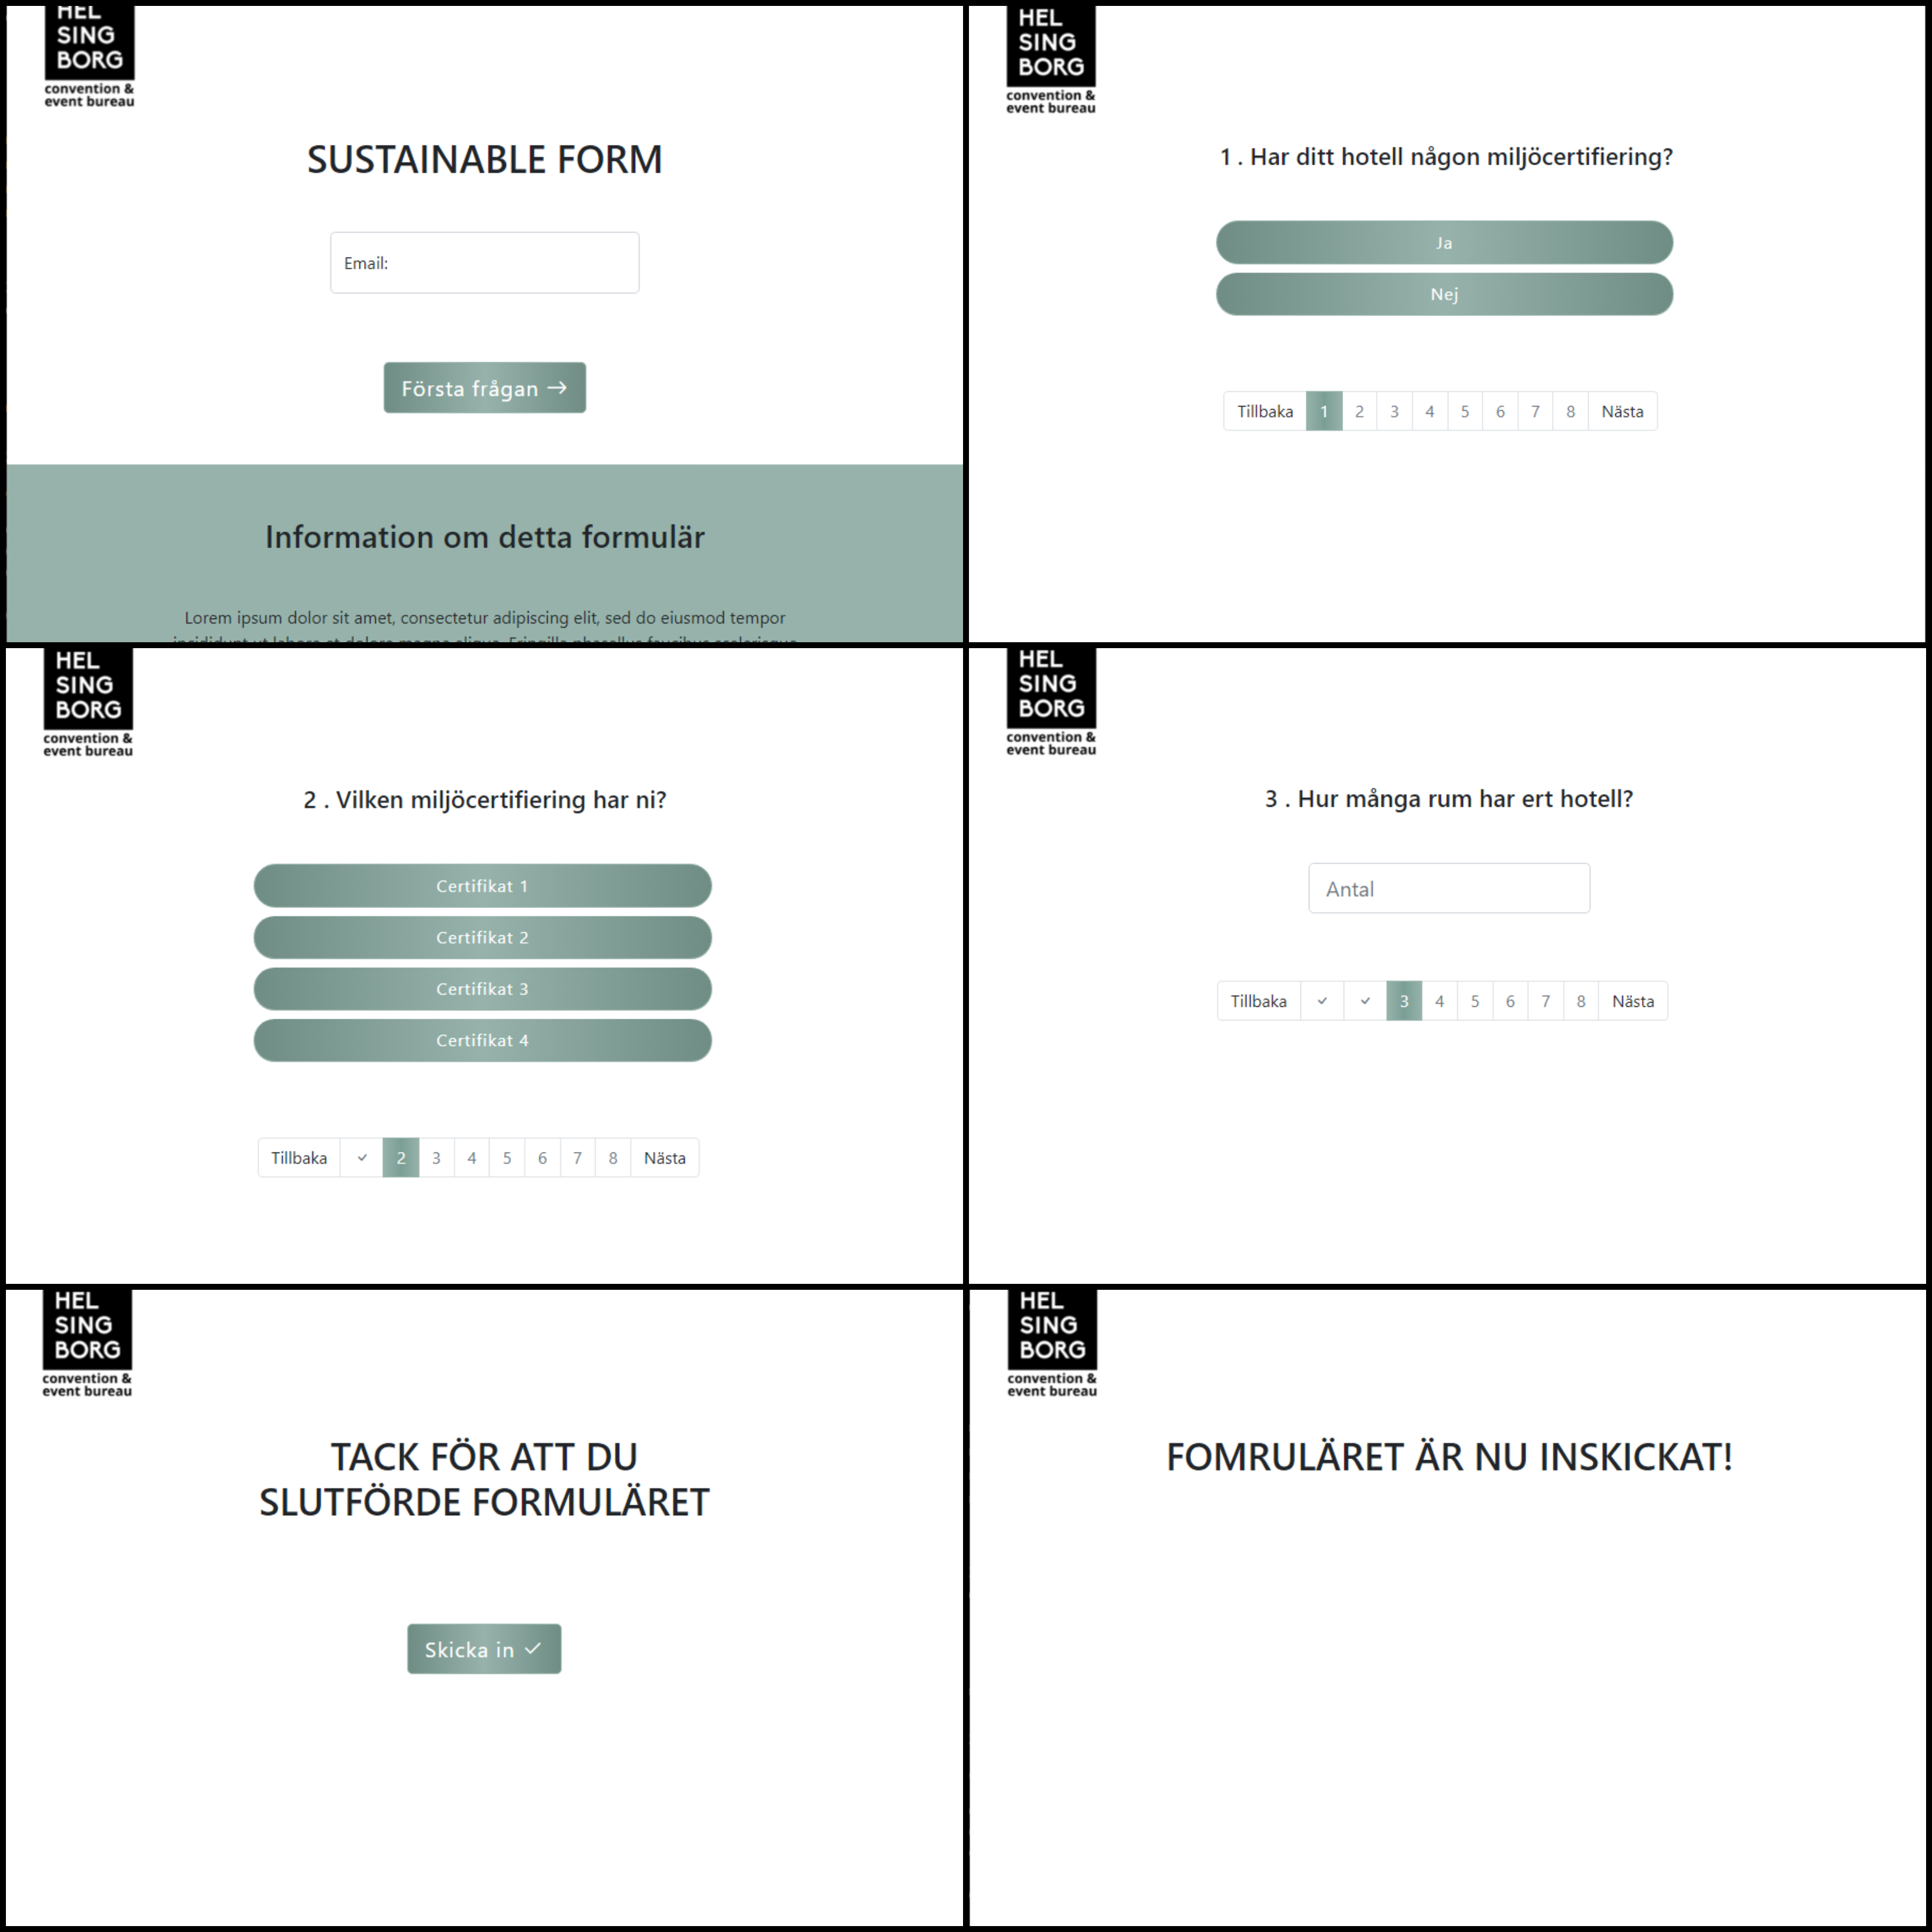
\includegraphics[width=140mm]{Proto-Coll-Q (1).jpg}
    \end{figure}
    \newpage
    \large{\textbf{R2.}}
    Administratörens sida som ingår i systemet ska ha ett utseende likt figur 2.
    \begin{figure}[h!]
        \centering
        \caption{Prototyp över administratörens sida}
        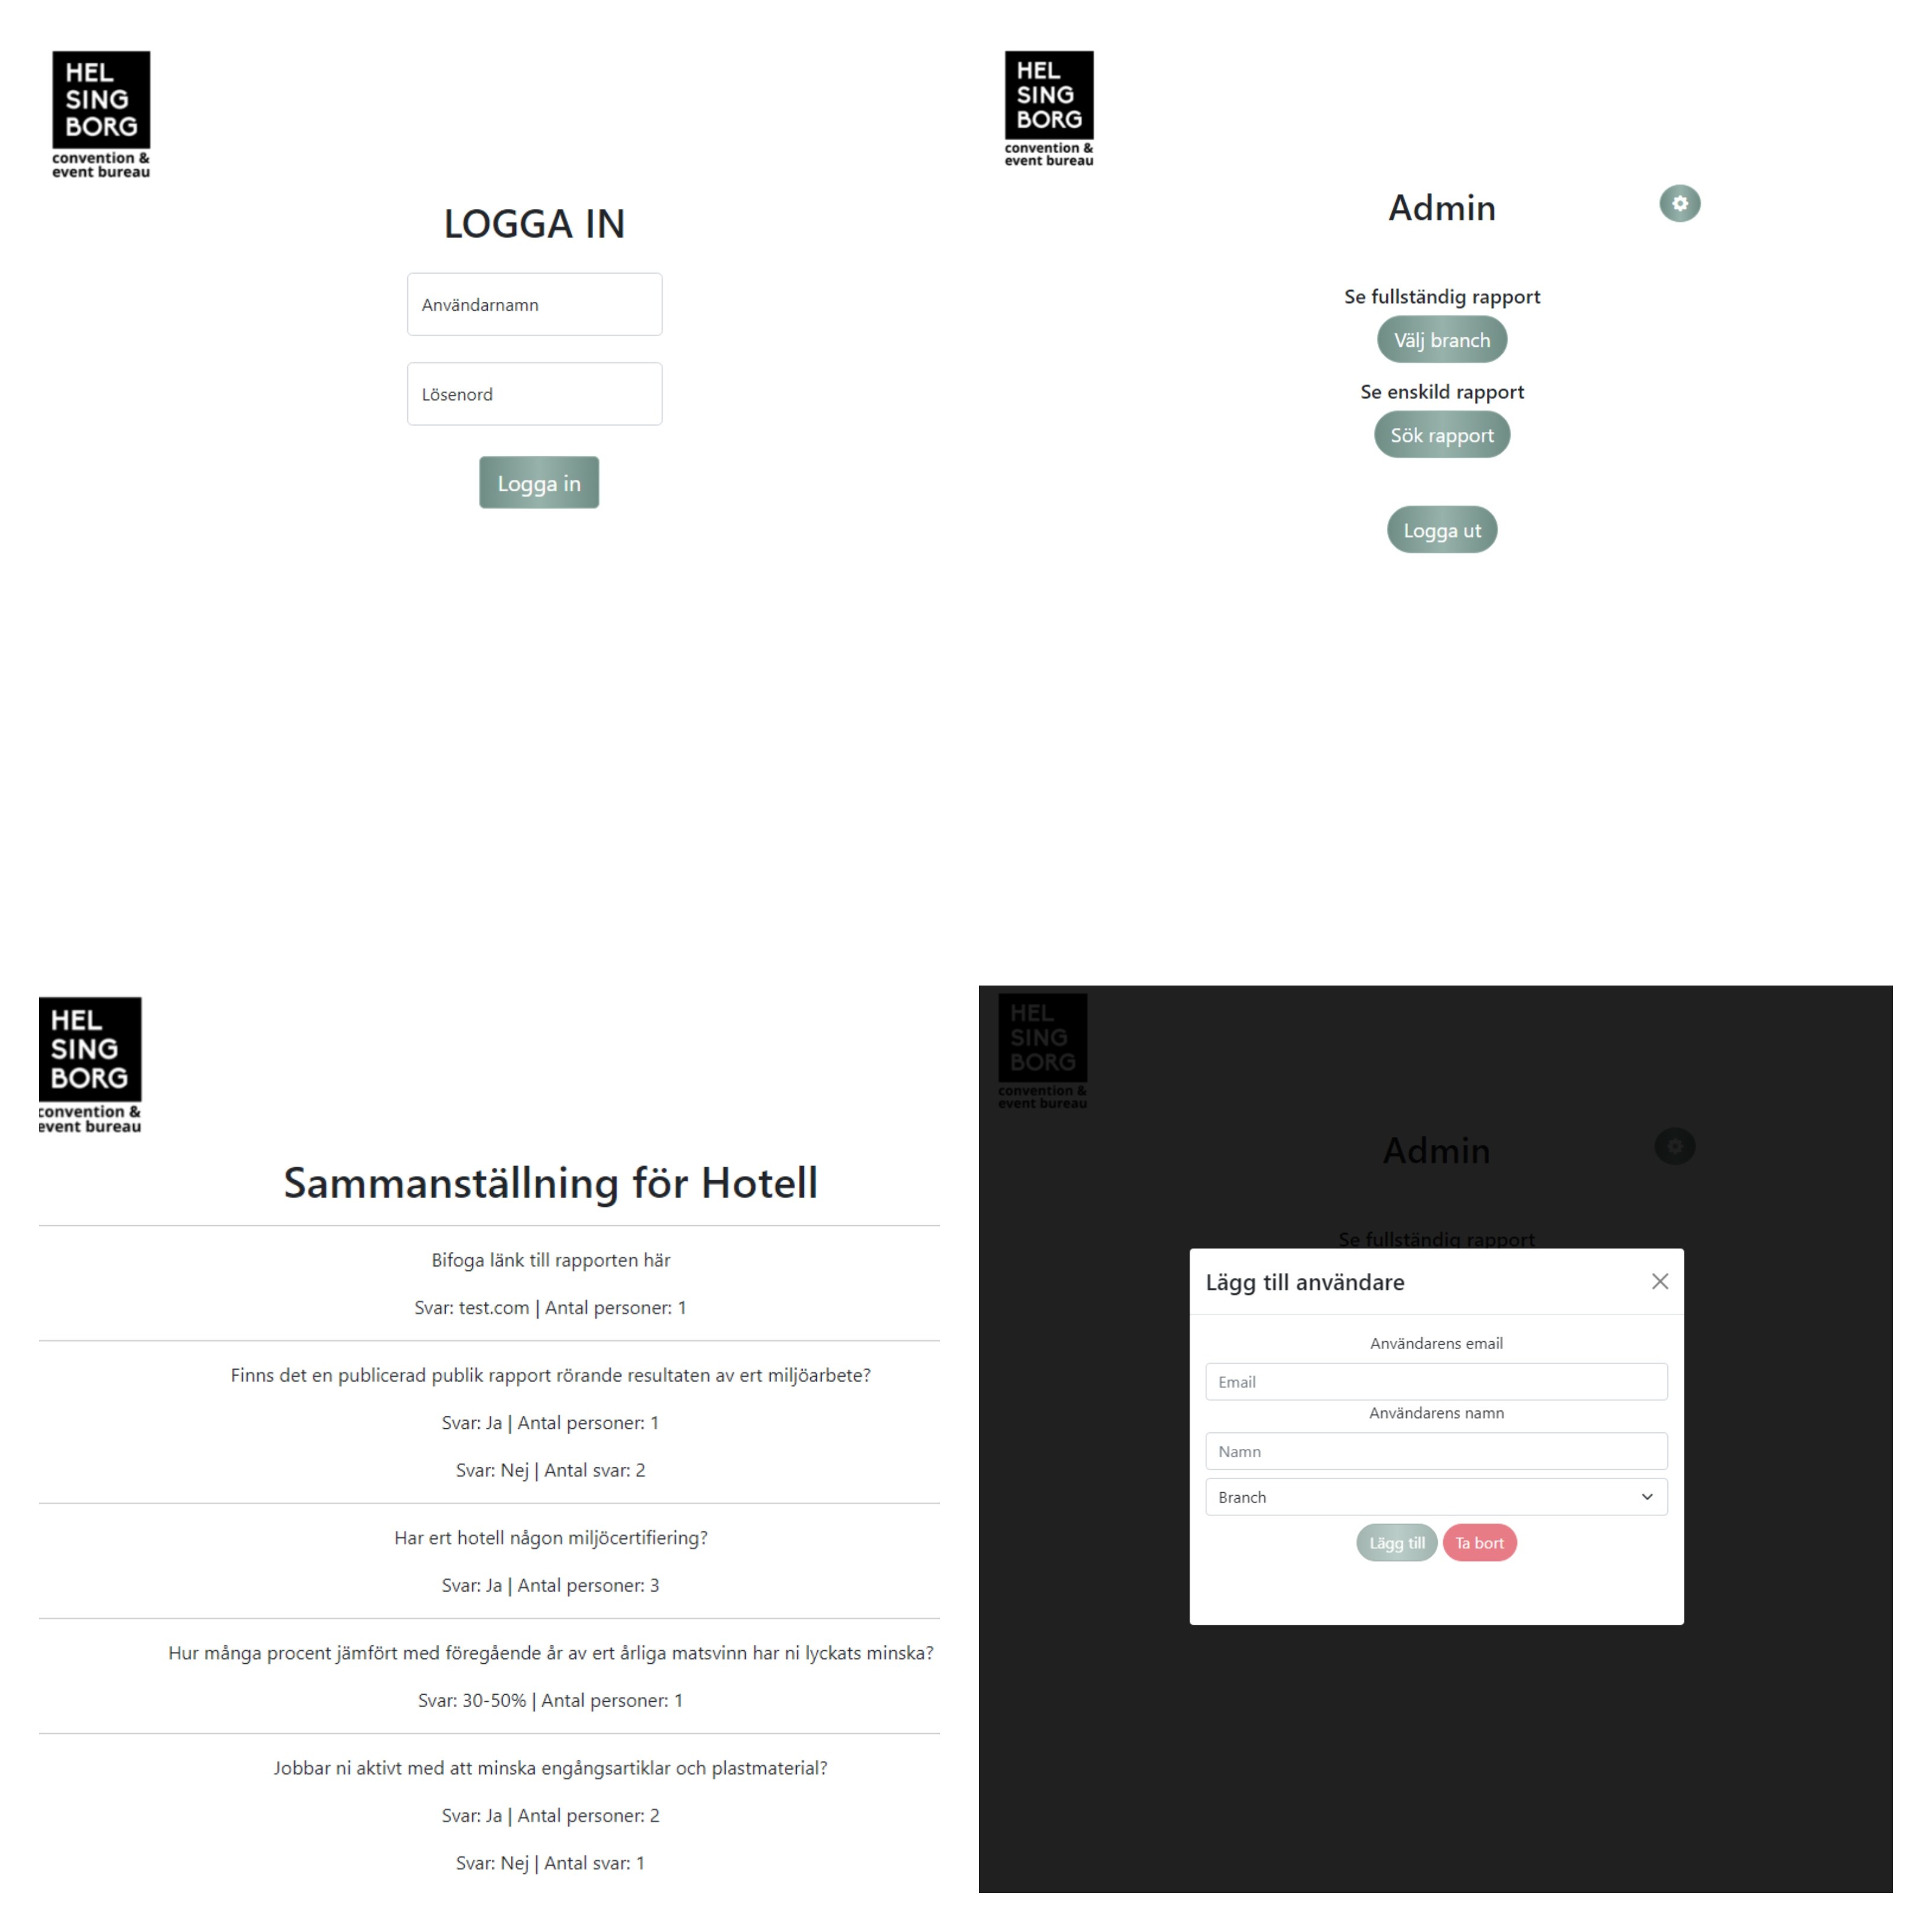
\includegraphics[width=140mm]{Proto-Coll-A.jpg}
        \label{fig:my_label}
    \end{figure}
\newpage
    
    \section{Hemsidans funktion}
\normalsize{Det här sektionen behandlar krav som är knutna till systemets funktionalitet. R3-R5 fokuserar på funktionaliteten som tillhör själva formuläret. R6 och R7 beskriver scenarior som ska gälla för administratören av systemet.
}
    \subsection{Stabila krav}
    
    \large{\textbf{R3.}}
    \normalsize{Följande scenario ska stödjas av systemet. \\
    \textbf{Scenario:} Svarspersonen navigerar till slutanvändarnas frågeformulär enligt figur 1.
        
    \noindent \textbf{Förutsättningar:} Svarspersonen har fått ett email från från HCEB. Mailet innehåller en länk till svarspersonenernas frågeformulär enligt figur 1.
        \begin{enumerate}
            \item Svarspersonen klickar på länken till formuläret som finns i mailet.
            \item Svarspersonen möts av formulärets startsida enligt figur 1 och ombeds mata in samma mailadressen som länken skickades till. 
        \end{enumerate}
}
\vspace{1em}

\noindent \large{\textbf{R4.}}
    \normalsize{Följande scenario ska stödjas av systemet. \\
    \textbf{Scenario:} Svarspersonen ska logga in på hemsidan med samma mailadress som mailet skickades till.
        \\
    \textbf{Förutsättningar:} Svarspersonen har fått en engångskod i samma mail som länken samt att svarspersonen befinner sig på startsidan.
        \begin{enumerate}
           \item Svarspersonen skriver in samma mailadress som mailet skickades till.
           \item Svarspersonen trycker på knappen "Första frågan" enligt figur 1.
           \item  Svarspersonen blir omdirigerad till första frågan enligt figur 1 och kan börja svara på formuläret.
        \end{enumerate}
   }
   
   \vspace{1em}
\noindent \large{\textbf{R5.}}
    \normalsize{Följande scenario ska stödjas av systemet.
        \\
       \textbf{Scenario:} Svarspersonen ska skicka in slutgiltig rapportering.
        \\
        \textbf{Förutsättningar:} Svarspersonen har svarat på samtliga frågor och befinner sig på sidan med den sista frågan enligt figur 1.
            \begin{enumerate}
                \item Svarspersonen svarar på sista frågan.
                \item Svarspersonen möts av en sidan med tack text enligt figur 1.
                \item Svarspersonen trycker på knappen "Skicka in".
                \item  Svarspersonen möts av en bekräftelsesida enligt figur 1 som bekräftar att formuläret är inskickat.
            \end{enumerate}
}

\vspace{1em}
\noindent \large{\textbf{R6.}}
    \normalsize{Följande scenario ska stödjas av systemet.
        \\
      \textbf{Scenario:} Administratören ska få tillgång till sammanställd data från en enskild bransch.
        \\
      \textbf{Förutsättningar:} Administratören är inloggad på admins hemsidan enligt figur 2.
            \begin{enumerate}
                \item Administratören trycker på knappen "Ladda ner" under rubriken "Ladda ner fullständig rapport".
                \item Administratören får upp en dropdown-meny med de olika branscherna.
                \item Administratören väljer den bransch som hen vill ha sammanställd data från.
                \item  Administratören dirigeras om vidare till en separat sida med data sammanställd från den bransch hen valde.
            \end{enumerate}
            
           } 
           \vspace{1em}
\noindent \large{\textbf{R7.}}
    \normalsize{Följande scenario ska stödjas av systemet.
        \\
       \textbf{Scenario:} Administratören ska få tillgång till sammanställd data från enskild aktör.
        \\
       \textbf{Förutsättningar:} Administratören är inloggad på admins hemsidan enligt figur 2.
            \begin{enumerate}
                \item Administratören trycker på knappen "Sök rapport" under rubriken "Ladda ner enskild rapport".
                \item Administratören får upp ett modal-fönster med en sökruta och en sök-knapp.
                \item Administratören skriver in namnet på den enskilda aktör hen vill söka efter.
                \item Administratören trycker på knappen med en sök ikon.
                \item  Administratören dirigeras om vidare till en separat sida med data sammanställd från den enskilda aktör hen valde.
            \end{enumerate}
    }
    
    \vspace{1em}

\subsection{Ändringsbenägna krav}
Dessa krav är hämtade från vår scrumboard. Eftersom vi först använde jira för att senare gå över till Trello så har vi två olika indexsystem: SF - X har sitt ursprung i Jiratiden och T - X kom till senare.

\subsubsection{Krav från scrumboard}
Krav \textit{SF-1} till och med \textit{SF-22} och \textit{T-1} till och med \textit{T-9} som finns på hemsidan \\ https://trello.com/b/DHOoURT9/sustainable-forms är även del av detta dokument.


    \subsection{Uteslutna krav}
       En del krav från vår scrumboard har blivit arkiverade så läsaren hänvisas dit.
     
    \newpage
     \section{Hemsidans hantering av data}
    
    \subsection{Stabila krav}
    \noindent \large{\textbf{R8.}}
    \normalsize{Systemet ska fungera enligt figur 2.
    
    \begin{figure}[h!]
    \caption{Kontext-diagram: Det utvecklade systemet innefattar \textit{Server, API, GUI} och \textit{Systemet}} och kommer hantera information mellan samtliga pilar exklusive kommunikationen mellan användare och HASAB.
    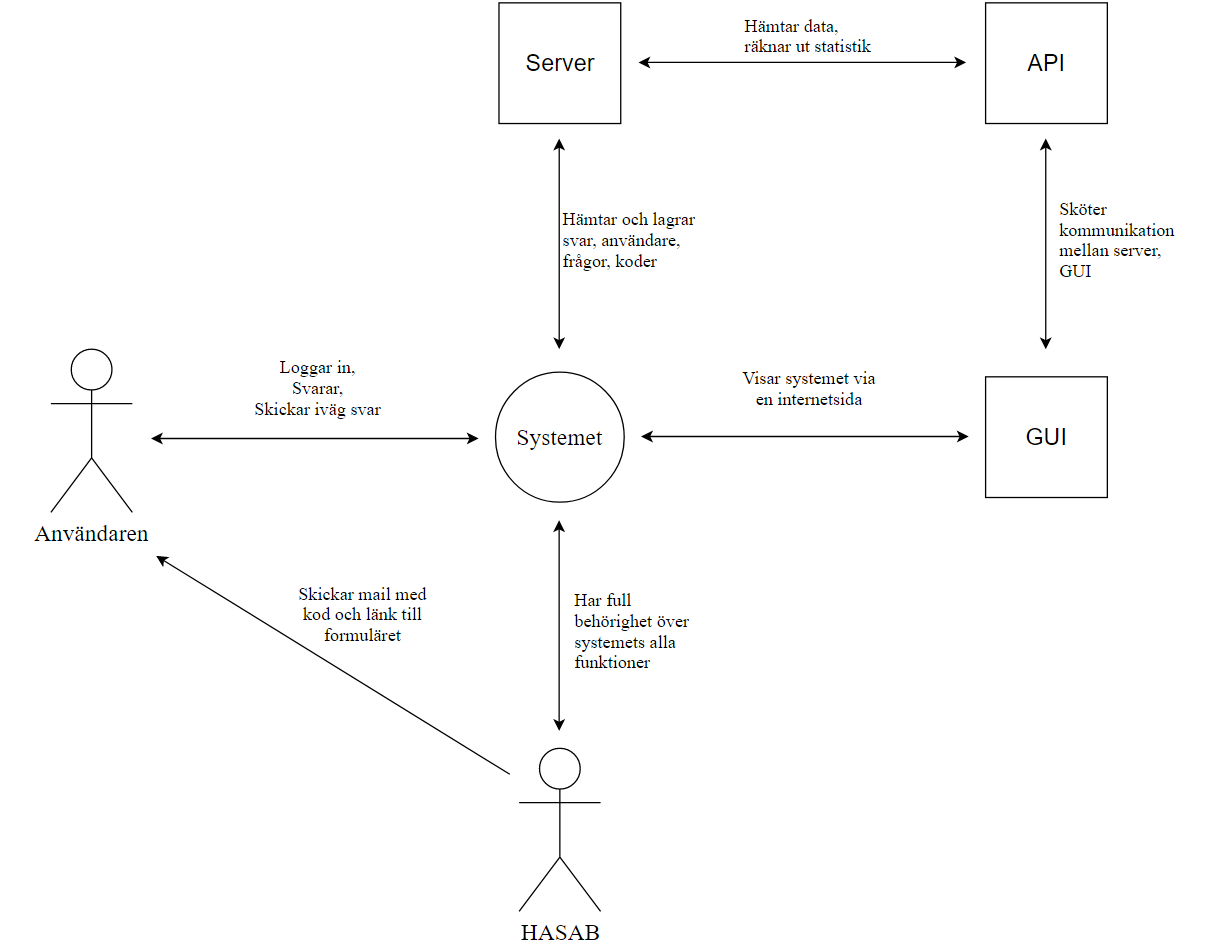
\includegraphics[width=150mm]{Kontextdiagram.png}
    
    \end{figure}
}
    \newpage
    \noindent \large{\textbf{R9.}}
    Systemet ska hantera data enligt figur 3.
       \begin{figure}[h!]
    
    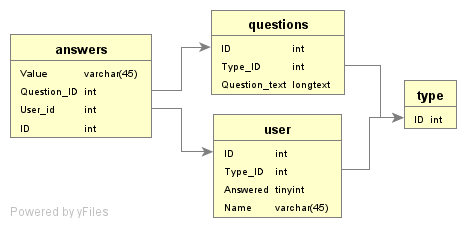
\includegraphics[width=150mm]{er.png}
    \caption{ER-diagram över datamodellen}
    \end{figure}
    
    
    \subsection{Ändringsbenägna krav och uteslutna krav}
    Även här hänvisas läsaren till scrumboarden.
    
  \newpage
   
    \section{Kvalitetskrav}
\normalsize{I den här sektionen presenteras krav som är relaterade till systemets användbarhet och användarupplevelse. Även krav kopplade till prestanda behandlas här.
}
    \subsection{Stabila krav}
    
  
\subsection{Ändringsbenägna krav}
     \noindent \large{\textbf{R10.}}
    \normalsize{Vid oförutsägbara händelser som påverkar systemets tillgänglighet ska en session sparas i 24 timmar från att den påbörjades.}

\vspace{1em}

    \noindent \large{\textbf{R11.}}
    \normalsize{Rapportering i systemet ska endast kunna göras av en användare som har fått tillgång till hemsidan via email.
    }
    
\vspace{1em}
\noindent \large{\textbf{R12.}}
    \normalsize{Fyra av fem svarspersoner ska anse att enkäten var lätt att svara på.
    
    }
    \vspace{1em}
    
\noindent \large{\textbf{R13.}}
\normalsize{En medelkunnig svarsperson ska kunna genomföra scenariot som beskrivs  \textbf{R2} och anlända till sidan inom 20 sekunder efter att de har klickat på länken.
    }
\vspace{1em}

\noindent \large{\textbf{R14.}}
    \normalsize{En medelkunnig slutanvändare ska kunna genomföra scenariot som beskrivs i \textbf{R3} inom en minut.
    }
    \vspace{1em}
    
\noindent \large{\textbf{R15.}}
    \normalsize{En medelkunnig slutanvändare ska kunna genomföra scenariot som beskrivs i \textbf{R4} inom 20 sekunder.
    }
    
    \vspace{1em}    
    \subsection{Uteslutna krav}
    De uteslutna kraven kan hittas på scrumboarden under arkiverade krav.
    \newpage
    \section{Leveranskrav}
    
    \subsection{Stabila krav}
\noindent \large{\textbf{R16.}}
     \normalsize{Leverans av en testbar version av systemet ska ske 2021-12-13. Vid leverans ingår en grundlig genomgång av systemet.
     }
\noindent \large{\textbf{R17.}}
     \normalsize{Vid första leverans enligt R16 skall en grundligt genomgång av systemet göras med kund. Denna genomgång kommer att ske under ett möte online.}
     
     \vspace{1em}
     

     
\noindent \large{\textbf{R18.}}
    \normalsize{Slutgiltig leverans av systemet ska ske 2022-01-20 och ska inkludera en fullt fungerande version av systemet.}
    
     
    \subsection{Ändringsbenägna krav}
    
    \noindent \large{\textbf{R19.}}
    \normalsize{Efter leveransen har skett och beställaren accepterat systemet har projektgruppen ingen möjlighet att ge teknisk support med tanke på att projektet ingår i en universitetskurs.}
    
    \subsection{Uteslutna krav}
    Läsaren hänvisas till scrumboarden.
    

\section{Sammanfattning}
Syftet med denna kravspecifikation är att beskriva det webbaserade rapporteringssystem som beställts av Helsingborg Convention and Event Bureau. Funktionella krav har presenterats, så som kravet på att tillgång till systemet ska ske genom en länk och att endast ifyllda formulär ska kunna skickas in. Andra krav har ett större fokus på svarspersonernas upplevelse och det faktum att ett enkelt gränssnitt och få valmöjligheter kan göra svarsprocessen mindre krävande. För ändringsbenägna och uteslutna krav hänvisas läsaren till projektets scrumboard. Avslutningsvis presenterades krav knutna till leveransen. 
    
    
   
\bibliographystyle{alpha}


\end{document}